\chapter{Introdução}
\label{cap:introducao}

O \textit{Node Package Manager} (\textit{npm}) é um gerenciador de pacotes para a linguagem \textit{JavaScript} e um registro\footnote{http://registry.npmjs.org/} no qual os pacotes publicados são armazenados. Lançado em 2009, seu principal objetivo é facilitar o compartilhamento de código escrito para o \textit{Node.js} e, atualmente, o registro do \textit{npm} ocupa a posição de maior repositório para uma dada linguagem, com mais de 1 milhão de pacotes.\footnote{http://www.modulecounts.com} O \textit{npm} é um dos que impulsionaram o \textit{JavaScript} a se tornar um ecossistema completo, com pacotes, \textit{frameworks}, aplicativos \textit{web} entre outros \cite{introduction:npm}. Além disso,  97\% dos aplicativos \textit{web} são oriundos do \textit{npm} \cite{stack_research}.

O \textit{npm} contém o maior número de dependências entre os diversos gerenciadores de pacotes para uma linguagem de programação \cite{teorical_reference:npm_2}. Nesse cenário, o termo \textit{provedor} refere-se ao pacote que provê recursos para os seus \textit{clientes}, que usufruem desses recursos, conforme definidos na Seção \ref{ref-teo:prov_clie}. Como há muitas dependências no \textit{npm}, quando algum provedor contém algum defeito, um grande número de clientes podem ser afetados, e foi exatamente isso que ocorreu no pacote chamado \textit{left-pad}.\footnote{https://blog.npmjs.org/post/141577284765/kik-left-pad-and-npm} Esse pacote foi removido do \textit{npm} e impactou milhares de outros pacotes em apenas 2,5 horas, incluindo pacotes renomados como o \textit{babel}\footnote{https://github.com/babel/babel} e o \textit{atom}\footnote{https://github.com/atom/atom} que por sua vez propagaram esse defeito para seus clientes. Assim, problemas entre provedores e clientes realmente ocorrem no ecossistema do \textit{npm} e por isso esse ecossistema foi escolhido como estudo de caso, devido ao número de dependências entre os pacotes.

As \textit{breaking changes}, descritas na Seção \ref{ref-teo:breaking_change}, são alterações nos provedores que os tornam incompatíveis com as suas versões anteriores \cite{intro:break_change}, fazendo com que os provedores tenham um comportamento inesperado. Um exemplo de \textit{breaking change} ocorreu no pacote \textit{optipng},\footnote{https://www.npmjs.com/package/optipng} no qual o método \textit{OptiPng.getBinaryPath} da versão \textit{0.1.1} foi renomado para \textit{OptiPng.getBinPath}\footnote{https://github.com/papandreou/node-optipng/compare/v0.1.1...v0.2.0\#diff-366460cd3c3170c9c84340631e6f8e4fL22-R19} na versão \textit{0.2.0}, fazendo com que todos os clientes que tinham acesso àquele método não o tivessem mais. Assim, o \cref{cod:bc:optipng} executa normalmente no cliente com o \textit{optipng@0.1.1}, mas ao atualizar para o \textit{optipng@0.2.0}, esse código deixa de funcionar devido à introdução de uma \textit{breaking change}.

\begin{lstlisting}[style=Javascript, label=cod:bc:optipng, caption={Código que sofre \textit{breaking change} do pacote \textit{optipng}}]
var OptiPng = require('optipng');
var cb = {apply: () => {}};
OptiPng.getBinaryPath(cb);
\end{lstlisting}

Apesar de ser um erro facilmente detectável pelo provedor, foi consertado somente após 34 dias, conforme mostra a Figura \ref{fig:bc_optipng}. Esta correção foi realizada em um \textit{commit}\footnote{https://github.com/papandreou/node-optipng/commit/a155f2b078224be18367847bbcbd3df3c379deea} no qual o desenvolvedor comentou que a renomeação do método ocorreu por engano.

\begin{figure}
    \centering
    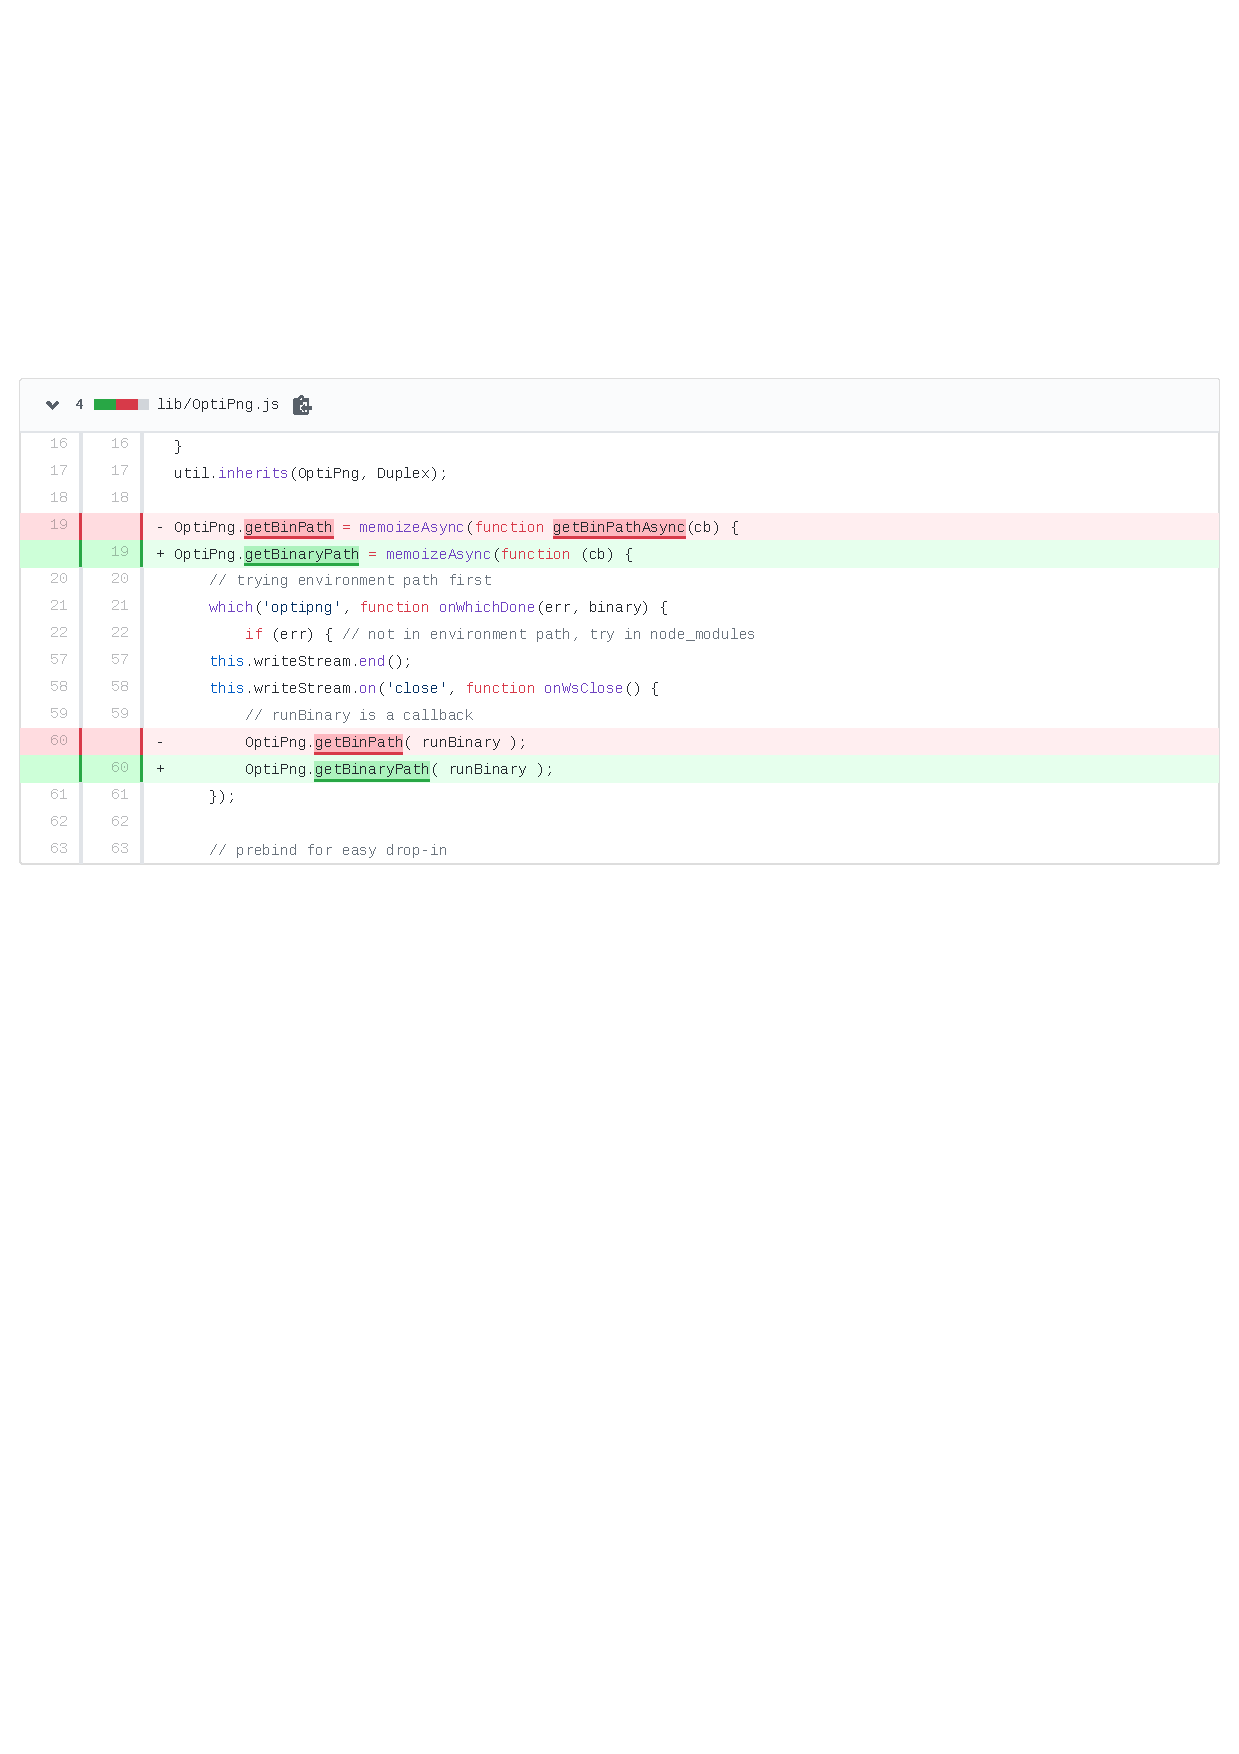
\includegraphics[scale=0.75]{figuras/bc_example.pdf}
    \caption{\textit{Commit} que corrigiu a \textit{breaking change}}
    \label{fig:bc_optipng}
\end{figure}{}

Além de quantificar as \textit{breaking changes} no ecossistema do \textit{npm}, este trabalho apresenta uma categorização das \textit{breaking changes} e de como os clientes se recuperam das \textit{breaking changes}. Para isso, foi utilizada uma amostra representativa dos clientes no \textit{npm} e, para cada uma de suas \textit{releases}, foi verificado se houve alteração nas \textit{releases} que os clientes aceitavam dos provedores. Então, determinou-se a versão do provedor que fora usada por cada cliente e os testes dos clientes executados através do comando \textit{npm test}. Após, foi analisada cada \textit{release} que resultou em erro para confirmar se o erro se tratava de uma \textit{breaking change} ou não. Por fim, foi feita uma análise nos repositórios dos provedores e dos clientes para recolher informações pertinentes a cada caso de \textit{breaking change}.

O Capítulo \ref{cap:ref-teorico} contém o referencial teórico desse trabalho. O Capítulo \ref{cap:qp} contém a motivação e o método para cada uma das questões de pesquisa. O Capítulo \ref{cap:metodologia} descreve a coleta dos dados que serão utilizados nessa pesquisa. O Capítulo \ref{cap:res_pre} apresenta os resultados preliminares da primeira e da segunda questão de pesquisa. Por fim, o Capítulo \ref{cap:cronograma} apresenta o cronograma previsto das atividades previstas para esse trabalho.

% isso estava nos results
%\filipe{o erro sempre se manifesta no cliente, acho que o lance é que você consegue identificar se o erro foi proveniente de uma chamada a uma função do provedor ou do próprio cliente (ou algum outro provedor que não interessa à análise).}

%\filipe{breaking change (defeito no provedor) vs. manifestação da breaking change (manifestação do defeito do provedor no cliente)}